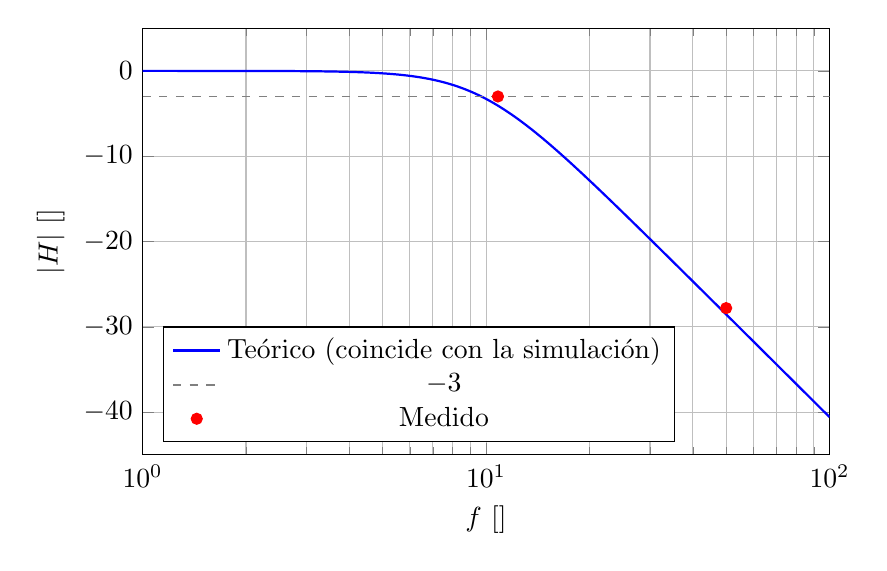
\begin{tikzpicture}
  \begin{axis}[
      width=0.85\textwidth, height=7cm,
      xmode=log, xmin=1, xmax=100, ymin=-45, ymax=5,
      xlabel={$f$ [\si{\hertz}]}, ylabel={$|H|$ [\si{\decibel}]},
      grid=both, legend pos=south west,
    ]
    % f0 = 9,675 Hz y Q = 0,709 con los valores comerciales
    % muestreo logarítmico: t = log10(f)
    \addplot[blue, thick, samples=200, domain=0:2]
      ({10^x}, {-10*log10((1 - (10^x/9.675)^2)^2 + (10^x/(9.675*0.709))^2)});
    \addlegendentry{Teórico (coincide con la simulación)}
    \addplot[gray, dashed, domain=1:100] {-3};
    \addlegendentry{$\SI{-3}{\decibel}$}
    \addplot[only marks, mark=*, red] coordinates {(10.83, -3) (50, -27.8)};
    \addlegendentry{Medido}
  \end{axis}
\end{tikzpicture}
